\subsection{The need for monotonicity in the unfolding}
\begin{example}\label{eq:twist}
    Consider the following elements in a second matrix power:
\begin{center}
\includegraphics[scale=.3, page=84]{pics.pdf}
\end{center}
Let $t_n \in \trees \mati 2 \rSigma$ be the tree which consists of a path with $n$ nodes using the unary label $a$, followed by a leaf with label $b$. If we apply term unfolding to this tree, and then project to the first coordinate, then we get a tree with a white leaf if and only if  $n$ is even.  If term unfolding were derivable, then thanks to the results from Section~\ref{sec:to-transductions}  we would get a first-order tree-to-tree transduction 
\begin{align*}
\trees \redset{a,b} \to \trees \rSigma
\end{align*}
where the output would contain a white leaf if and only if the input has odd depth. This is in turn would imply that having even depth for trees over $\redset{a,b}$ is first-order definable, which it is not, because first-order logic cannot do modulo counting.
\end{example}
The problem in the above example is that the letter $a$ does a swap on its ports, which leads to counting modulo two. To forbid such swaps, we impose a monotonicity requirement that matches the monotonicity requirement for register updates in register transducers.
